\documentclass{beamer}

\usepackage[utf8]{inputenc}
%\usepackage[scaled]{uarial} % not available in Linux
\renewcommand{\rmdefault}{phv} % Arial

\renewcommand{\sfdefault}{phv} % Arial
\renewcommand*\familydefault{\sfdefault} %% Only if the base font of the document is to be sans serif

\usepackage[T1]{fontenc}
\usepackage{classico}

\title{Classificazione dei bosoni elettrodeboli con una rete neurale al Large Hadron Collider} 
\subtitle{6 Novembre 2024}
\date{6 Novembre 2024}
\author{Jacopo Lancione}

\usetheme{UNITO}
    %\setbeamercovered{invisible} %default
    \setbeamercovered{transparent} % Items to be uncovered already visible, but almost transparent
    
\begin{document}
\begin{frame}
    \titlepage
\end{frame}

\begin{frame}{Sommario}
    \tableofcontents
\end{frame}


\section{Introduzione}
\subsection{LHC}
\begin{frame}{Large Hadron Collider - CMS}
  \includegraphics[width=.1\linewidth]{./cern_logo.pdf}
  \includegraphics[width=.1\linewidth]{./cms_logo.pdf}
  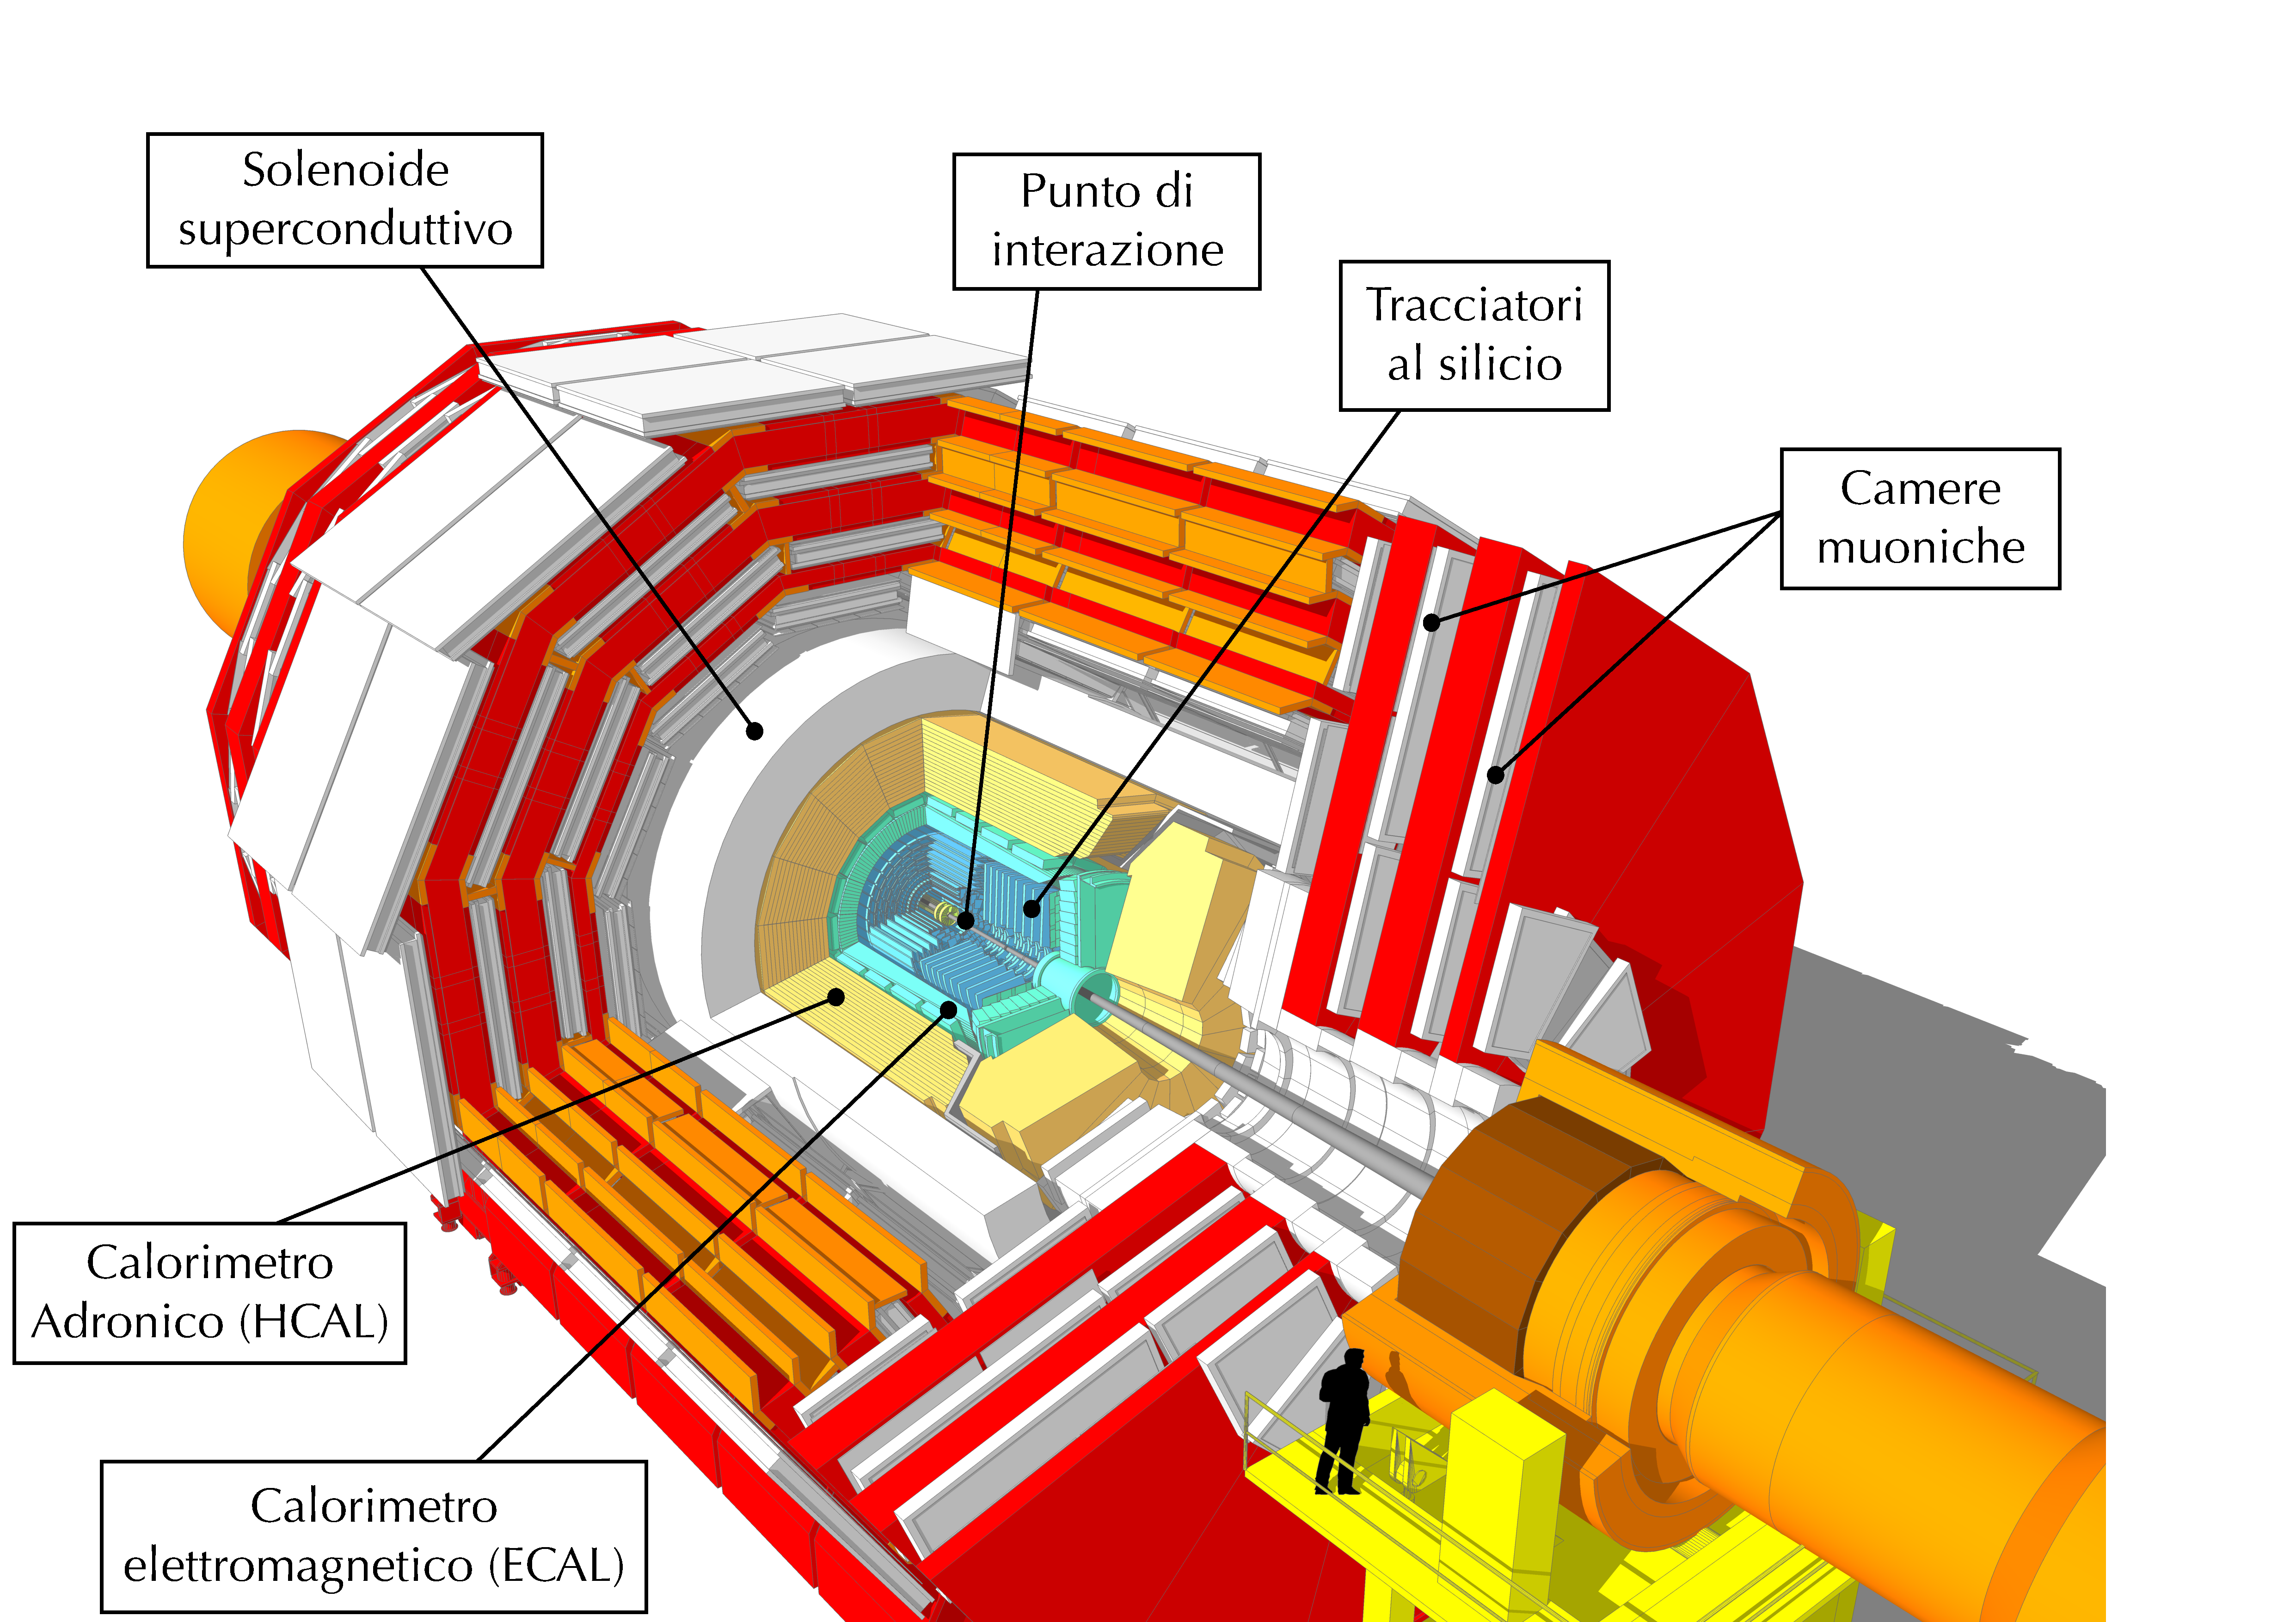
\includegraphics[width=.4\linewidth]{./cms_cutaway.pdf}
  % https://cds.cern.ch/record/2665537

  {\scriptsize
  L'anello di accelerazione + grande del mondo, parliamo del CMS da cui arrivano i miei dati, in cui si producono particelle in abbondanza,

  (foto del cern e dl cms)

  Del CMS mi interessa giusto introdurre il fatto che ci siano dei calorimetri perché alcuni loro parametri sono tra le features (differenze tra i calorimetri)

  Si produce un enorme mole di dati e per trattarli si utilizzano anche tecniche di machine learning (e così passo alla prox slide)

  E posso accennare molto rapidamente al Nobel di quest'anno (fallo!!)
  }
\end{frame}

\subsection{Machine Learning}
\begin{frame}
  \vspace*{-3ex}
  \begin{figure}
    \centering
    \resizebox{\linewidth}{!}{
      \begin{tikzpicture}[mindmap, outer sep=0pt,
        level 1 concept/.append style={level distance=148},
        level 2 concept/.append style={level distance=120},
        text=white,
        decoration={start radius=1cm, end radius=.5cm,amplitude=2mm,angle=30}]%,

        \only<-2>{
          \node [circle, minimum width=3.2cm, fill=unitocolor] (ml) at (0,0) {\huge\color{white}Machine\\[.5ex] Learning}
            child [grow=-10]
              {node [circle, minimum width=3.3cm, fill=unitograyA!60] (unsup) {\Large \!\!\!\!\!\!Unsupervised Learning}
                child [grow=-40]{ node[circle, minimum width=2.5cm, fill=unitocolor](clust)  {\normalsize Clustering}}
                child [grow=-85]{ node[circle, minimum width=2.5cm, fill=unitocolor](reduct) {\normalsize Riduzione dimensionale}}
              }
            child [grow=190] 
              {node [circle, minimum width=3.3cm, fill=unitograyA!60] (sup) {\Large Supervised Learning}
                child [grow=220]{ node[circle, minimum width=2.5cm, fill=unitocolor](classif) {\normalsize Classifi\-cazione}}
                child [grow=-95]{ node[circle, minimum width=2.5cm, fill=unitocolor](regr)    {\normalsize \!\!\!Regressione}}
          };
        }
        \only<3>{
          \node [circle, minimum width=3.2cm, fill=unitocolor] (ml) at (0,0) {\huge\color{white}Machine\\[.5ex] Learning}
            child [grow=-10]
              {node [circle, minimum width=3.3cm, fill=unitograyA!60] (unsup) {\Large \!\!\!\!\!\!Unsupervised Learning}
                child [grow=-40]{ node[circle, minimum width=2.5cm, fill=unitocolor](clust)  {\normalsize Clustering}}
                child [grow=-85]{ node[circle, minimum width=2.5cm, fill=unitocolor](reduct) {\normalsize Riduzione dimensionale}}
              }
            child [grow=190] 
              {node [circle, minimum width=3.3cm, fill=unitograyA!60] (sup) {\Large Supervised Learning}
                child [grow=220]{ node[circle, minimum width=2.5cm, fill=faircolor](classif) {\normalsize\color{black} Classifi\-cazione}}
                child [grow=-95]{ node[circle, minimum width=2.5cm, fill=unitocolor](regr)    {\normalsize \!\!\!Regressione}}
            };
          }

        \path (ml) to[circle connection bar switch color=from (unitocolor) to (unitograyA!60)] (unsup);
        \path (ml) to[circle connection bar switch color=from (unitocolor) to (unitograyA!60)] (sup);
        \path (unsup) to[circle connection bar switch color=from (unitograyA!60) to (unitocolor)] (clust);
        \path (unsup) to[circle connection bar switch color=from (unitograyA!60) to (unitocolor)] (reduct);
        \only<-2>{
          \path (sup) to[circle connection bar switch color=from (unitograyA!60) to (unitocolor)] (classif);
        }
        \only<3>{
          \path (sup) to[circle connection bar switch color=from (unitograyA!60) to (faircolor)] (classif);
        }
        \path (sup) to[circle connection bar switch color=from (unitograyA!60) to (unitocolor)] (regr);

        \node [inner sep=0pt, text width=6.5cm, minimum height=4.5cm] (nobel) at ($(ml) - (0,5.5)$) {
          \only<2->{
            \includegraphics[width=\textwidth]{./nobel_prize.jpeg}
          }
        };
      \end{tikzpicture}
    }
  \end{figure}
%
% {\scriptsize
%   In questa slide devo far passare il concetto di labeled e unlabeled data (posso anche metterle come item)
% }

% {\scriptsize
%   Qua dicendo che il mio progetto ruota attorno ad un problema di classificazione passo alla prox slide
% }
\end{frame}

\begin{frame}{Il Progetto di tesi}
% {\scriptsize
%   Che sia chiaro dove si colloca il mio progetto:
%   affrontare un problema di classificazione binaria (logistic regression), nell'ambito della Fisica delle alte energie
%
%   Immagine classica del modello std e 1 di 1 rete neurale giusto per dire rapidamente il Cosa e il Come
%
%   il mio obiettivo: allenare 1 rete che distingua al meglio tra i 2 canali di decadimento
% }
  \vspace*{-3.5ex}
  \begin{center}
    \Large
    Classificare
  \end{center}
  \vspace*{-1.5ex}
  \begin{columns}[T]
    \column{.40\linewidth}
      \begin{block}{}
        \centering%
        Bosoni elettrodeboli
      \end{block}
      \begin{figure}
        \centering
        \includegraphics[width=\textwidth]{./sm_overview.pdf}
      \end{figure}

    \column{.11\linewidth}
      {
        \setbeamercolor{block body}{bg=white, fg=black}
        \begin{block}{}
          \centering\small
          con una
        \end{block}
      }
    \column{.35\linewidth}
      \begin{block}{}
        \centering
        Rete neurale
      \end{block}
      \parbox[t][][c]{\textwidth}{
        \vspace*{3ex}
        \centering
        \includegraphics[width=.9\textwidth]{./nn_diagram.pdf}
      }
  \end{columns}
\end{frame}

\section{Dataset}
\begin{frame}
  \centering
  \Huge\bfseries
  Il Dataset
\end{frame}

\subsection{Decadimenti dei bosoni}
\begin{frame}{Decadimenti di $Z$ e $W$}
  Diciamo subito qlche dettaglio in $+$ sul dataset (e magari mettiamolo anche a fondo slide, il riferimento a dove ho scaricato i dati)

  qua posso mettere i diagrammi di Feynman dei decadimenti, giusto per mettere qualcosa sotto gli occhi al pubblico

  Elencare le features ie la cinematica di interesse e anche le variabili lasciate da parte in riferimento al rivelatore

% Ql è in breve la fisica del processo
  \vfill
  \begin{flushright}
    \scriptsize
    https://opendata.cern.ch/record/545
  \end{flushright}
\end{frame}

\subsection{Preprocessing}
\begin{frame}{Preprocessing}

  {\scriptsize
  Racconto di come ho trattato i dati: la storia del chi2 (vogliamo dirla? nn ne conosco i dettagli purtroppo), la qstione dgli outlier

  Qua mostriamo sicuramente i pairplot che sono la cosa più indicativa, magari anche i boxplot? -> in questa maniera escono $+$ slides (e qua posso sprecarmi con il logaritmo e lo questione del'approccio scartato con le sigma)
  
  Raccontiamo la storia di correlazioni evidenti che permetterebbero una facile classificazione, nel caso $+$ semplice attraverso 1 appl lineare

  I concetti da far passare sono 2: è meglio è avere 1 dataset uniforme, quindi scaliamo tutto e ci sbarazziamo degli outlier, evitare di introdurre ridondanze (ie guardare in faccia i dati con pairplot)
  }
\end{frame}

\section{Reti Neurali}
\subsection{Architettura e principi}
\begin{frame}
  \centering
  \Huge\bfseries
  Reti Neurali
\end{frame}

\begin{frame}{L'architettura}
  % sicuramente la platea apprezza la concisione ie qnte info riesco a far passare nel minor tempo a patto di 1 buona qltà dl'info
  Qua bisogna introdurre i parametri su cui ho agito: numero di layer, nodi, attivazione, algoritmo di ottimizzazione (questo nella slide successiva)

  E devo spiegare come funziona la questione dei parametri (pesi e bias) e dove si introduce la non linearità (attivazione)

  Questa slide la organizzerei come un elenco .ntato a sx e una bella immagine con cui io riesca a spiegare tutto 
\end{frame}

\begin{frame}{Loss function \\Algoritmi di ottimizzazione}
  % Qsto per spiegare come funzioni la rete, nn per mostrare risultati ancora
  L'idea di 1 loss function da minimizzare (come se fosse un'energia), qsta nn è semplice da spiegare visivamente, di questa metterei proprio la formula così la commento un attimo

  Algoritmo (sarebbe carino accennare al learning rate e al momento e all'adattività degli algoritmi)


  Immagini di allenamenti significativi, magari anche in cui si veda l'overfitting

\end{frame}

\subsection{Risultati dell'allenamento}
\begin{frame}{Risultati}
  E qua ci va una carrellata di rock curves che può tranquillamente occupare $+$ slides, quali voglio scegliere come significative? Con algoritmi diversi e mostrando bene il test point

\end{frame}



\begin{frame}{Conclusioni}
  \begin{itemize}
    \item Le reti neurali si prestano molto bene a compiti di particle identification
    \item Sono degli strumenti molto flessibili e quindi il mio progetto è facilmente generalizzabile ad altre necessità/misure
    \item Ho identificato una classe di modelli equivalenti
  \end{itemize}
  \vspace{2ex}

  studi futuri: provare a combinare i dataset e allenare una rete su quelli per distinguere i bosoni uno dall'altro

    \vspace*{4ex}
    \begin{columns}
      \column{.4\linewidth}
      {
        \only<1>{\setbeamercolor{block body}{bg=white, fg=white}}
        \begin{block}{}
          \centering\vspace*{1ex}
          \only<1>{}
          \only<2>{
            \Large\bfseries
            \color{white}
            Grazie a tutti!%
          }%
        \vspace*{1ex}
      \end{block}
      }
    \end{columns}
\end{frame}

\end{document}
